\chapter{Intelligenza Artificiale}\index{Intelligenza Artificiale}
\section{Cenni storici}
La nascita ufficiale dell’Intelligenza Artificiale viene collocata nel 1956 per un convegno al college di Hanover organizzato da John McCarthy\index{McCarthy, John}, al quale erano presenti Minsky, Shannon, Newell, Simon e molti altri pionieri dell’informatica. Alla base del seminario era la congettura che ogni aspetto dell’apprendimento e ogni caratteristica dell’intelligenza possa, in linea di principio, essere descritto in modo talmente preciso da renderlo simulabile da una macchina.

In questo senso l’informatica fornisce la metafora computazionale per lo studio della mente; l’Intelligenza Artificiale invece ha permesso di unificare con una metodologia comune tutte le discipline della scienza cognitiva, introducendo l’idea di lavorare con simboli che non necessariamente rappresentano dei numeri interessandosi di attività ritenute tipicamente umane.

A seguito della nascita dell’IA, nei successivi anni, si sono sviluppate due principali correnti di pensiero, quella \emph{hard} e quella \emph{soft}.

\section{Intelligenza Artificiale hard e soft}
L’intelligenza artificiale hard si concentra sulle attività ritenute tipicamente umane come la dimostrazione automatica di teoremi, la risoluzione di problemi e i giochi, senza preoccuparsi del modo in cui vengono ottenuti tali risultati, ma solo di ottenerli e renderli rapidi, precisi e a prova d’errore.

Dalla parte opposta, invece, la corrente dell’IA soft tiene sempre come riferimento l’uomo. Il suo obiettivo è quello di riprodurre per mezzo del calcolatore i processi mentali umani e quindi il corrispondente comportamento. La caratteristica fondamentale è l’importanza che viene data al procedimento rispetto ai risultati finali. Il criterio di successo di una simulazione, quindi, consiste nella più stretta somiglianza possibile con il corrispondente modo umano di elaborare. Questi rigidi vincoli devono produrre un risultato identico, e non migliore, rispetto a quello umano. In questo senso, sarà importante riprodurre anche gli eventuali errori che compie l’essere umano nella simulazione artificiale.

\begin{table}[hbt]
\centering
  \begin{tabularx}{\textwidth}{*3{>{\centering\arraybackslash}X}}
    & \textbf{IA hard} & \textbf{IA soft} \\
    \hline
    Risultati (rispetto all'uomo) & Uguali o migliori & Uguali\\
    Procedure (rispetto all'uomo)& Nessun vincolo purché efficienti & Identiche \\
    Errori & Da evitare & Da riprodurre
  \end{tabularx}
  \caption{Differenze tra IA hard e soft}
\end{table}

\section{Perché un programma?}
Secondo l’approccio computazionale, la parte essenziale di un’attività mentale può essere riprodotta da un programma di calcolo. La costruzione di un programma che simula l’attività mentale introduce criteri operativi di scientificità diversi da quelli basati sull’osservabilità.

La realizzazione di questo programma permette:
\begin{itemize}
  \item di esplicitare completamente la teoria e la sua non-contraddittorietà (in modo non assoluto, ma rispetto alla parzialità del modello);
  \item di essere riproducibile, anche se la funzione mentale in oggetto resta inosservabile;
  \item di essere falsificabile, ovvero un comportamento del programma al di fuori dell’aspettativa confuta la teoria che sta simulando (Lakatos, 1970);
  \item di essere un efficiente e veloce generatore di previsioni, di calcoli e di test;
  \item di controllare il tempo per farlo scorrere più lentamente o più velocemente, al fine di osservare fenomeni o processi evolutivi inosservabili per l’uomo in condizioni normali (ad esempio, l’evoluzione dal bambino all’adulto).
\end{itemize}

\section{Falsificabilità}
Il \emph{principio di falsificabilità}\index{principio di falsificabilità}\index{falsificabilità|see{principio di falsificabilità}} è stato elaborato nel 1959 da Karl Popper\index{Popper, Karl}\footnote{Sir Karl Raimund Popper (Vienna, 28 luglio 1902 – Londra, 17 settembre 1994) è stato un filosofo e epistemologo austriaco naturalizzato britannico. Popper è anche considerato un filosofo politico di statura considerevole, difensore della democrazia e del liberalismo e avversario di ogni forma di totalitarismo. Egli è noto per il rifiuto e la critica dell'induzione, la proposta della falsificabilità come criterio di demarcazione tra scienza e non scienza, la difesa della ``società aperta''.} in \emph{Logic of scientific discovery}. Il criterio di falsificabilità afferma che una teoria, per essere controllabile, e perciò scientifica, deve essere ``falsificabile'': in termini logici, dalle sue premesse di base devono poter essere deducibili le condizioni di almeno un esperimento che la possa dimostrare integralmente falsa alla prova dei fatti, secondo il procedimento logico del \emph{modus tollens} (in base a cui, se da A si deduce B, e B è falso, allora è falso anche A)\footnote{Formalmente, $((p \to q) \land \neg q) \to \neg p) $}. Se una teoria non possiede questa proprietà, è impossibile controllare la validità del suo contenuto informativo relativamente alla realtà che essa presume di descrivere.

\section{Validazione di una teoria}\index{validazione di una teoria}
In generale, se sulla base di una teoria data non è possibile generare un programma per calcolatore che riproduca gli aspetti essenziali della teoria stessa, allora la teoria non è scientificamente accettabile. Il fallimento della simulazione diventa quindi indice di contraddizioni, incompletezze o ambiguità che possono gettare dubbi sulla teoria della validità. D’altra parte anche stabilire quando una simulazione ha avuto successo non è sempre ovvio, ed è legato al problema di quanto possa essere spinta la somiglianza fra l’uomo e la macchina.

Secondo la scienza cognitiva, la validazione di una teoria segue una metodologia in diversi passi di esecuzione, come mostrato nella figura \ref{fig:validazioneTeoria}.

\begin{figure}[hbt]
  \centering
  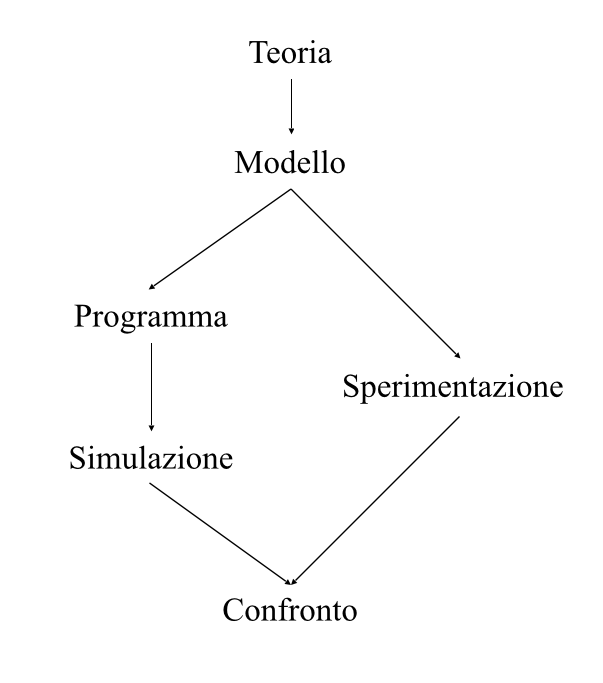
\includegraphics[width=0.5\textwidth]{img/validazioneTeoria}
  \caption{Processo di validazione di una teoria}
  \label{fig:validazioneTeoria}
\end{figure}

\begin{enumerate}
  \item \emph{Derivazione del modello dalla teoria}. La teoria ha una portata superiore a qualsiasi realizzazione empirica. Un modello è un’interpretazione particolare di una teoria e da una di queste si possono generare più modelli.
  \item \emph{Creazione del programma dal modello}. Un programma di calcolo equivalente al modello viene creato. I dettagli implementativi non dovrebbero influenzare la simulazione, ma nella pratica già la scelta del linguaggio condiziona il programma e quindi la simulazione.
  \item \emph{Sperimentazione e simulazione}. In questa fase le previsioni della teoria vengono testate sulla base di sperimentazioni di laboratorio su soggetti umani e simulazioni computazionali. Qui inizia per la teoria la possibilità di essere falsificata. Se i risultati sperimentali sono differenti da quelli previsti, la teoria deve riuscire a spiegare il perché della discrepanza.
  \item \emph{Confronto}. Questa fase corrisponde al confronto tra i risultati della sperimentazione e quelli della simulazione. Se si verifica una piena congruenza fra i risultati della simulazione e quelli della sperimentazione è stata ottenuta una validazione computaizonale.
\end{enumerate}

Per la verifica e la validazione di una teoria sono necessari due criteri. Il criterio di identità dei risultati finali vincola il programma a riprodurre le prestazioni ottenute dagli esseri umani impegnate nello stesso compito. Questo criterio è necessario ma non sufficiente, gli si deve aggiungere quello di \emph{equivalenza delle procedure}.\index{equivalenza delle procedure}

Dal momento che le procedure non sono direttamente osservabili, si deve decidere come si possa controllare il criterio di equivalenza. Zenon Pylyshyn\index{Pylyshyn, Zenon}, nel 1984, suggerì di prendere in considerazione gli stadi di elaborazione intermedi prima del risultato e i tempi di risposta. Il programma deve quindi simulare gli stati rilevanti di conoscenza, che corrispondono agli stadi di elaborazione intermedi fra stato iniziale e finale. Ad esempio, se gli esseri umani risolvono un problema in 3 passi, anche la macchina deve riprodurre i passi intermedi e non solo la soluzione finale. Inoltre, il tempo di computazione del programma deve essere proporzionale al tempo di computazione necessario ai soggetti umani per eseguire una certa operazione. Questa proporzionalità si deve estendere non solo ai risultati finali, ma anche agli stati rilevanti intermedi.

Tutti i passi qui sopra delineati vanno considerati bidirezionali, nel senso che in ogni fase ci sono feedback verso l’alto che tendono a modificare la teoria, il modello e il programma di calcolo sulla base dei risultati sperimentali.

Alla luce di ciò l’intelligenza artificiale soft va considerata come lo strumento base che consente alla scienza cognitiva di analizzare i procedimenti simulati dalla macchina, confrontandoli con quelli messi in atto dalla mente umana.

\section{Le reti neurali}\index{rete neurale}\label{reti-neurali}
L’approccio classico dell’intelligenza artificiale utilizza l’architettura classica dei calcolatori, ovvero quella proposta da John von Neumann. Questa architettura usa una memoria statica contenente le informazioni e una unità di elaborazione centrale che opera sui dati attivi.

I primi a proporre una valida alternativa a questa architettura furono McCulloch e Pitts in un famoso lavoro del 1943, \emph{A logical calculus of the ideas immanent in nervous activity}, il quale schematizza un combinatore lineare a soglia, con dati binari multipli in entrata e un singolo dato binario in uscita: un numero opportuno di tali elementi, connessi in modo da formare una rete, è in grado di calcolare semplici funzioni booleane.

F. Rosenblatt nel libro \emph{Phychological review} introduce il primo schema di rete neurale, detto \emph{percettrone}\index{percettrone}, antesignano delle attuali reti neurali, per il riconoscimento e la classificazione di forme, allo scopo di fornire un'interpretazione dell'organizzazione generale dei sistemi biologici. Il modello probabilistico di Rosenblatt è quindi mirato all'analisi, in forma matematica, di funzioni quali l'immagazzinamento delle informazioni, e della loro influenza sul riconoscimento dei pattern; esso costituisce un progresso decisivo rispetto al modello binario di McCulloch e Pitts, perché i suoi pesi sinaptici sono variabili e quindi il percettrone è in grado di apprendere.

L'opera di Rosenblatt stimola una quantità di studi e ricerche che dura per un decennio, e suscita un vivo interesse e notevoli aspettative nella comunità scientifica, destinate tuttavia ad essere notevolmente ridimensionate nel 1969 da Marvin Minsky\index{Minsky, Marvin} e Seymour A. Papert, nell'opera \emph{An introduction to computational geometry}, nella quale mostrano i limiti operativi delle semplici reti a due strati basate sul percettrone, e dimostrano l'impossibilità di risolvere per questa via molte classi di problemi, ossia tutti quelli non caratterizzati da separabilità lineare delle soluzioni. Questo tipo di rete neurale non è abbastanza potente: non è infatti neanche in grado di calcolare la funzione or esclusivo (\texttt{XOR}).

\subsection{Implementazione e apprendimento}
Il funzionamento di una rete neurale è in linea di principio molto semplice. Le \emph{unità di input} rappresentano l’ingresso del sistema: il loro stato di attivazione dipende dagli stimoli esterni alla rete. Le unità interne, dette \emph{hidden}, ricevono segnali dalle unità di input e se attivate ritrasmettono a quelle successive attraverso le connessioni disponibili. Le \emph{unità di output} determinano la risposta allo stimolo ricevuto inizialmente.

\begin{figure}[hbt]
  \centering
  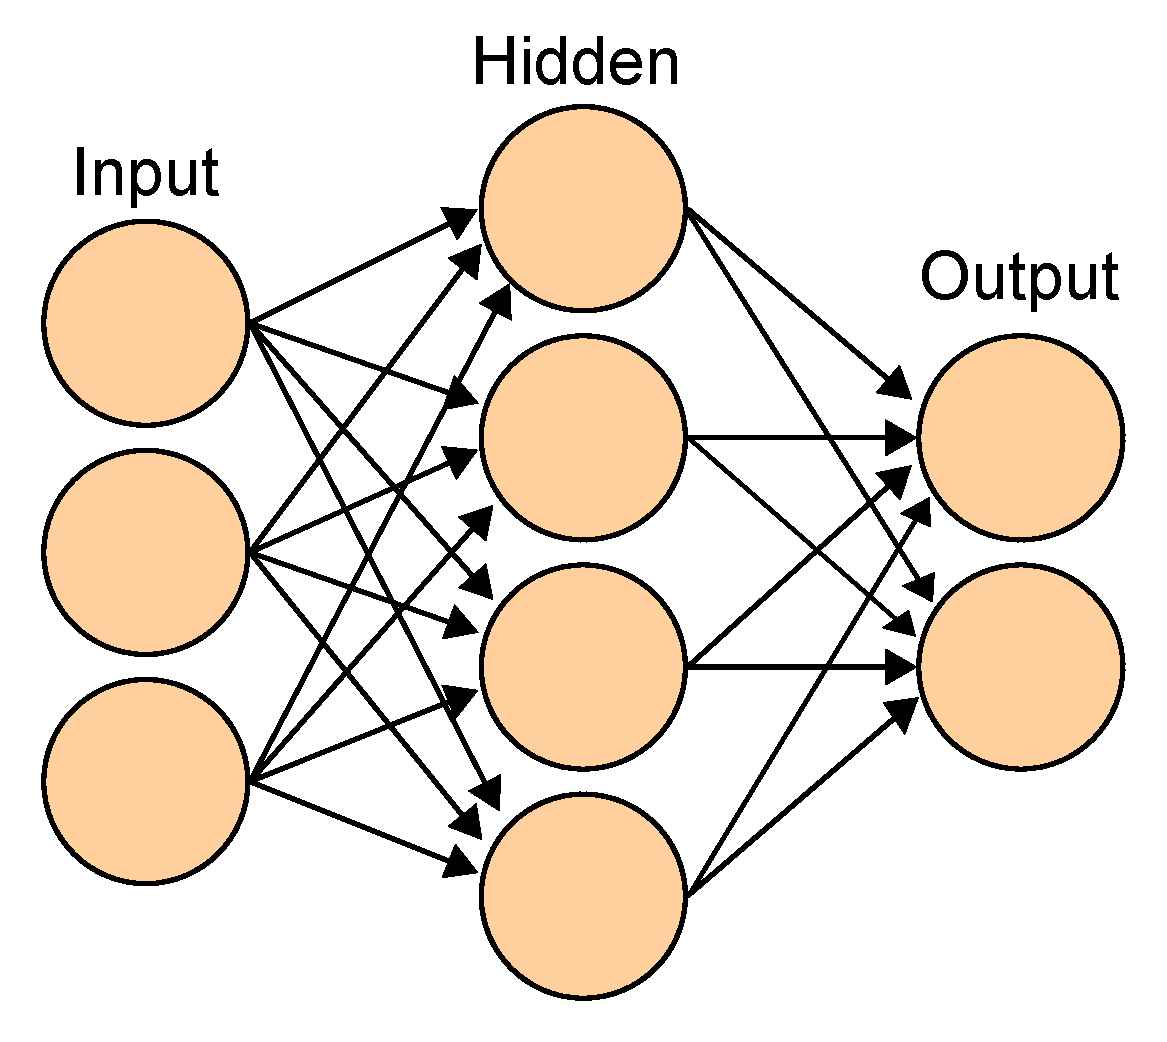
\includegraphics[width=.5\textwidth]{img/Artificial_neural_network}
  \caption{Semplice esempio di rete neurale}
  \label{fig:rete-neurale}
\end{figure}

Il contesto matematico per addestrare le reti MLP (Multi-Layers Perceptron, ossia percettrone multistrato) fu stabilito dal matematico americano Paul Werbos nella sua tesi di dottorato del 1974. Uno dei metodi più noti ed efficaci per l'addestramento di tale classe di reti neurali è il cosiddetto algoritmo di \emph{retropropagazione dell'errore} (error backpropagation), proposto nel 1986 da David E. Rumelhart, G. Hinton e R. J. Williams, il quale modifica sistematicamente i pesi delle connessioni tra i nodi, così che la risposta della rete si avvicini sempre di più a quella desiderata. Tale lavoro fu prodotto riprendendo il modello creato da Werbos. L'algoritmo di backpropagation è una tecnica d'apprendimento tramite esempi, costituente una generalizzazione dell'algoritmo d'apprendimento per il percettrone sviluppato da Rosenblatt nei primi anni Sessanta. Mediante questa tecnica era possibile, come detto, trattare unicamente applicazioni caratterizzabili come funzioni booleane linearmente separabili.

Le reti neurali, assieme alla logica fuzzy e agli algoritmi genetici, hanno aperto la strada a quello che viene definito il \emph{soft computing}, ovvero quelle tecniche che si prefiggono di valutare, decidere, controllare e calcolare in un ambito impreciso e vago ed emulando e utilizzando la capacità degli esseri umani, di eseguire le suddette attività sulla base della loro esperienza.

\section{Limiti dell'Intelligenza Artificiale}
I limiti dell’IA possono essere differenziati in tecnologici, metodologici e di etica scientifica. I limiti tecnologici derivano dai vincoli imposti da hardware e software disponibili. Una possibile soluzione è quella di una forte parallelizzazione computazionale; in generale il limite tecnologico è ben definito ed in costante regresso.

Più stringenti sono i limiti intrinseci nel metodo computazionale, in quanto insuperabili in linea di principio. Questi derivano dalla definizione classica che accomuna uomo e calcolatore, considerati macchine per l’elaborazione di simboli dotati di significato. È importante distinguere in questo caso delle differenze tra il cervello umano e quello artificiale nei termini della capacità di manipolare i simboli e di relazionarsi con il mondo.

La critica alla metafora del computer è esplicitata da John Searle\index{Searle, John}\footnote{John Rogers Searle (Denver, 31 luglio 1932) è un filosofo statunitense. Professore di filosofia all'Università della California, a Berkeley, è noto per i suoi contributi alla filosofia del linguaggio e alla filosofia della mente. Ha ricevuto il premio Jean Nicod nel 2000.} nel 1980, con il suo esperimento mentale sulla camera cinese\index{camera cinese}. Alla base del ragionamento di Searle è che la sintassi (grammatica) non è equivalente alla semantica (significato). I sostenitori dell'intelligenza artificiale forte sostengono che un computer opportunamente programmato non sia solo la simulazione o un modello della mente, ma che esso possa essere una mente. Esso cioè capisce, ha condizioni conoscitive e può pensare. L'argomento di Searle (o meglio, l'esperimento mentale) si oppone a questa posizione. L'argomentazione della stanza cinese è la seguente:

\begin{quotation}\small
  «Si supponga che, nel futuro, si possa costruire un computer che si comporti come se capisse il cinese. In altre parole, il computer prenderebbe dei simboli cinesi in ingresso, eseguirebbe un programma e produrrebbe altri simboli cinesi in uscita. Si supponga che il comportamento di questo computer sia così convincente da poter facilmente superare il test di Turing. In altre parole, il computer possa convincere un uomo che parla correttamente cinese (per esempio un cinese) di parlare con un altro uomo che parla correttamente cinese, mentre in realtà sta parlando con un calcolatore. A tutte le domande dell'umano il computer risponderebbe appropriatamente, in modo che l'umano si convinca di parlare con un altro umano che parla correttamente cinese. I sostenitori dell'intelligenza artificiale forte concludono che il computer capisce la lingua cinese, come farebbe una persona, in quanto non c'è nessuna differenza tra il comportamento della macchina e di un uomo che conosce il cinese.

Ora, Searle chiede di supporre che lui si sieda all'interno del calcolatore. In altre parole, egli si immagina in una piccola stanza (la stanza cinese) con un libro contenente la versione in inglese del programma utilizzato dal computer e carta e penna in abbondanza. Searle potrebbe ricevere scritte in cinese attraverso una finestra di ingresso, elaborarle seguendo le istruzioni del programma, e produrre altri simboli cinesi in uscita, in modo identico a quanto faceva il calcolatore. Searle fa notare che egli non capisce i simboli cinesi. Quindi la sua mancanza di comprensione dimostra che il calcolatore non può comprendere il cinese, poiché esso è nella sua stessa situazione. Il calcolatore è un semplice manipolatore di simboli, esattamente come lo è lui nella stanza cinese - e quindi i calcolatori non capiscono quello che stanno dicendo tanto quanto lui.»
\end{quotation}

Il punto della dimostrazione di Searle è che la macchina si limita a manipolare simboli, senza poterli interpretare, e quindi senza mai avere accesso al loro significato nel mondo. In questo senso la macchina può simulare stati intenzionali, ma non può possederli. Può comportarsi come se avesse stati mentali, ma non agire in presa diretta sul mondo, come fanno gli esseri umani, in quanto dotati materialmente di cervello. La conclusione che se ne può trarre è che la macchina, a meno di riprodurre completamente anche il substrato biologico del cervello umano, non può generare imitazioni complete, ma solo simulazioni parziali dei processi mentali. La macchina non ha accesso ai significati, ma solo ai loro simboli, mentre l’uomo manipola i simboli avendo contemporaneamente accesso ai loro significati nel mondo.
